\documentclass{beamer}
\usetheme{Berlin}
\usepackage[utf8]{inputenc}
\usepackage[english, serbianc]{babel}
\usepackage{multicol}
\usepackage{booktabs}
\usepackage{multimedia}

\titlegraphic{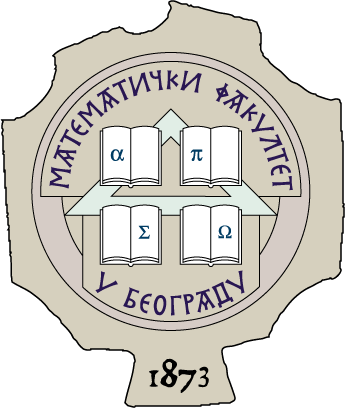
\includegraphics[height=2cm]{img/matf-logo.png}} 

\setbeamerfont{title}{size=\large}
\setbeamerfont{subtitle}{size=\small}
\setbeamerfont{author}{size=\small}
\setbeamerfont{date}{size=\small}
\setbeamerfont{institute}{size=\small}
\title{Мастер рад}
\subtitle{Примена неуронских поља зрачења у рендеровању}  %% Change project title here
\author{Коста Грујчић} %% Change author name here
\institute{Универзитет у Београду, Математички факултет}
\date[\textcolor{white}{\today}]  %% Change presentation date here
{\today}

\newtheorem{myDef}{Дефиниција}

\begin{document}
	\frame[plain]{\titlepage}
	
	\section{Увод}
		\begin{frame}{Основни појмови}
			\begin{myDef}
				Рендеровање је поступак којим се од тродимензионе сцене добија слика.
			\end{myDef}
		
			\begin{myDef}
				Поље је пресликавање $F:\mathbb{R}^n \rightarrow \mathbb{R}^m$.
			\end{myDef}
		\end{frame}

		\begin{frame}{Тачкасти модел камере}
			\begin{center}
				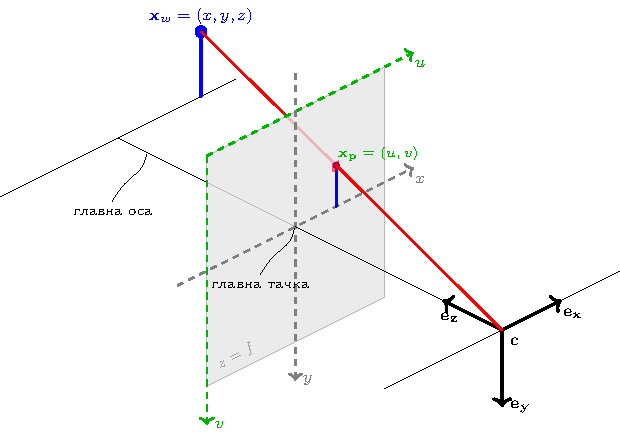
\includegraphics[width=0.8\textwidth]{img/pinhole.pdf}
			\end{center}
		\end{frame}
	
		\begin{frame}{Запреминско рендеровање}
			\begin{equation*}
				C(\Pi_{\mathbf{r_{c, d}}}) = \int_{t_n}^{t_f}T(t)\sigma(\mathbf{r_{c, d}}(t))C(\mathbf{r_{c, d}}(t))dt,
			\end{equation*}
			где jе $\Pi_{\mathbf{r_{c, d}}}$ тачка пресека светлосног зрака и равни слике, а $C$ поље које сваку тачку
			пресликава у њену RGB боју, а $T(t)=\exp{\left(-\int_{t_n}^{t}\sigma(\mathbf{r_{c, d}}(s))ds\right)}$
			aкумулирана пропусност зрака.
		\end{frame}
	
		\begin{frame}{Неуронске мреже}
			\begin{center}
				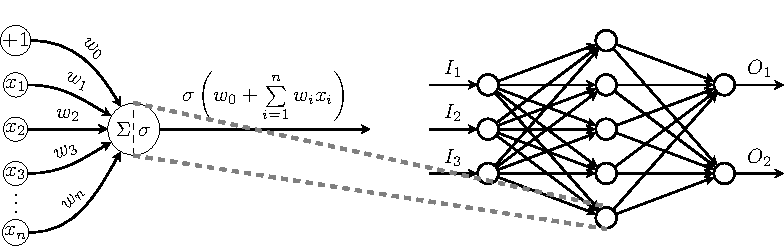
\includegraphics[width=\textwidth]{img/mlp.pdf}
			\end{center}
		\end{frame}
	
	\section{Архитектуре}
		\begin{frame}{NeRF}
			\begin{center}
				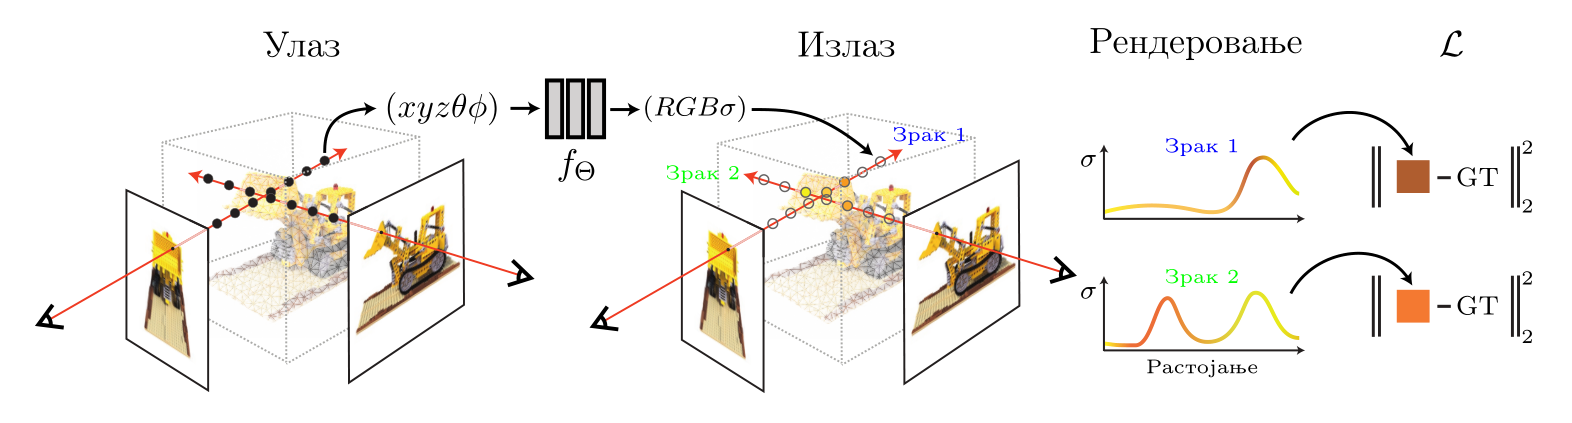
\includegraphics[width=1\textwidth]{img/img/nerf-ss.png}
			\end{center}
		\end{frame}
	
		\begin{frame}{Фуријеизација}
			Неуронску мрежу $F_\Theta$ можемо видети као композицију $F_\Theta^\prime \circ \gamma$ где се $\gamma$
			не обучава. У овом случају је $\gamma : \mathbb{R} \rightarrow \mathbb{R}^{2D}$ и то конкретно
			
			\begin{equation*}
				\gamma(x) = (\sin(2^0\pi x), \cos(2^0 \pi x), ..., \sin(2^{D-1}\pi x), \cos(2^{D-1}\pi x)).
				\label{eqn-fourier-features}
			\end{equation*}
		\end{frame}
		
		\begin{frame}{mip-NeRF}
			\begin{center}
				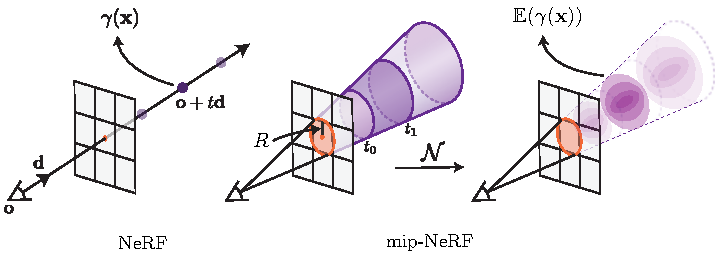
\includegraphics[width=0.9\textwidth]{img/mipnerf.pdf}
			\end{center}
		\end{frame}
		
		\begin{frame}{Ref-NeRF}
			\begin{center}
				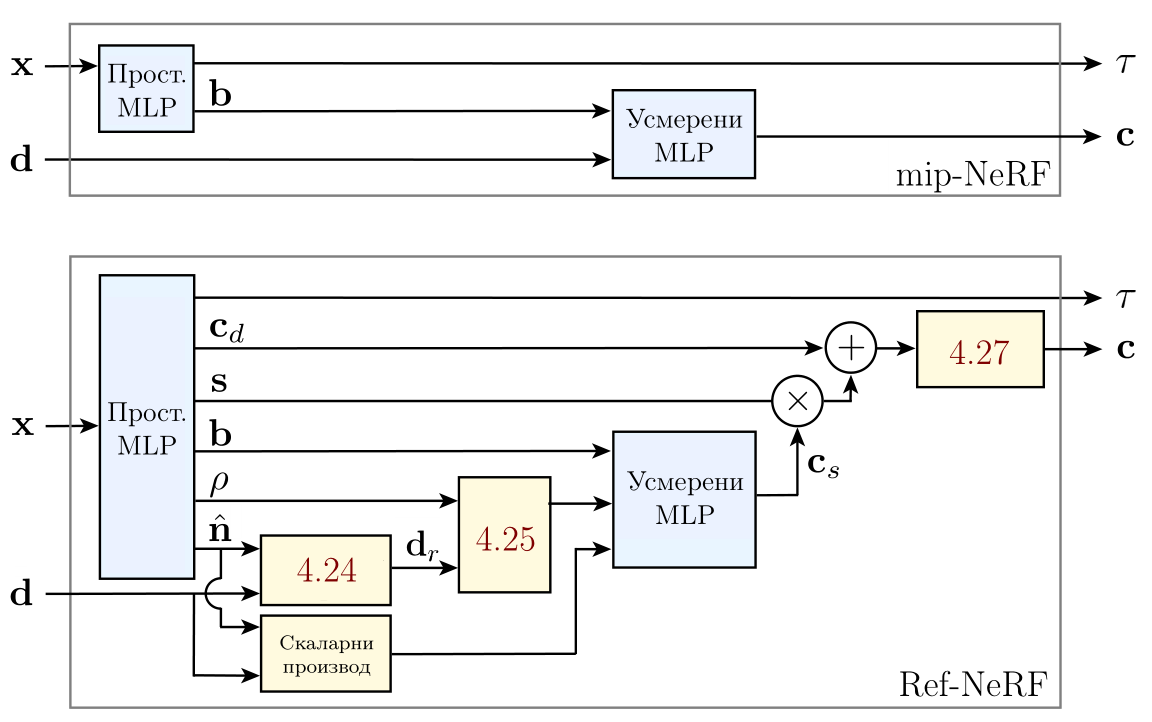
\includegraphics[width=0.9\textwidth]{img/img/refnerf-ss.png}
			\end{center}
		\end{frame}

	\section{Подаци}
		\begin{frame}{Подаци}
			\begin{itemize}
				\item Референтни скупови података
				\item Синтетички
			\end{itemize}
		\end{frame}

		\begin{frame}{Скупови података}
			\begin{figure}
				\centering
				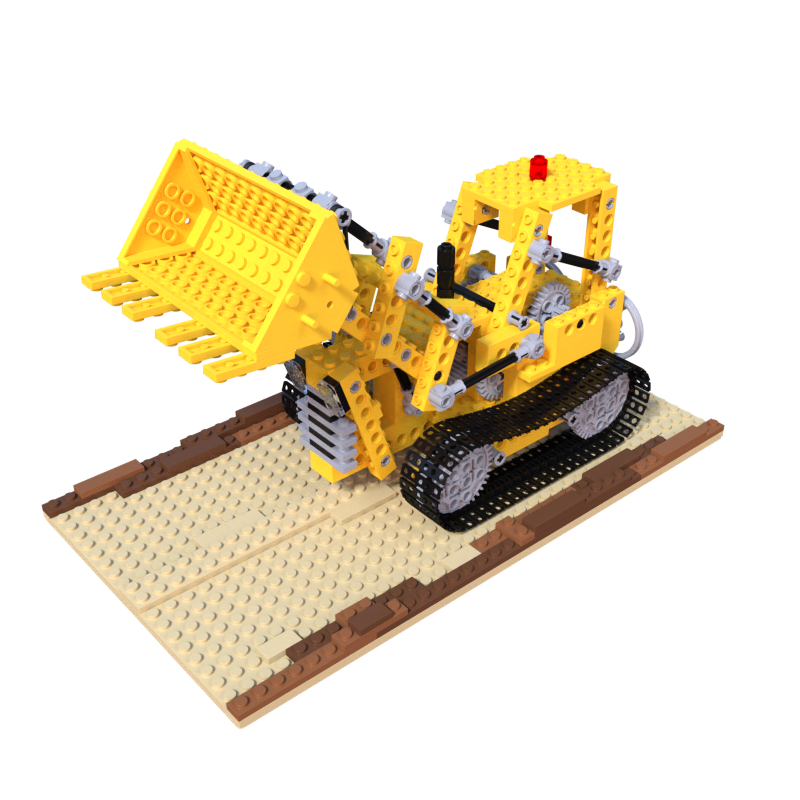
\includegraphics[width=.3\textwidth]{img/lego_gt.png}\quad
				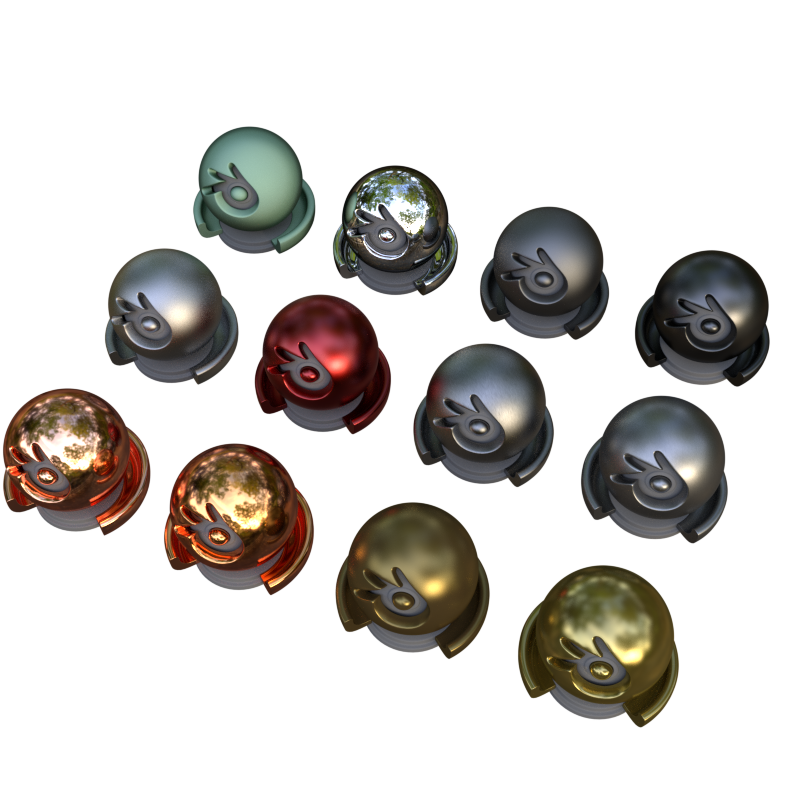
\includegraphics[width=.3\textwidth]{img/materials_gt.png}\quad
				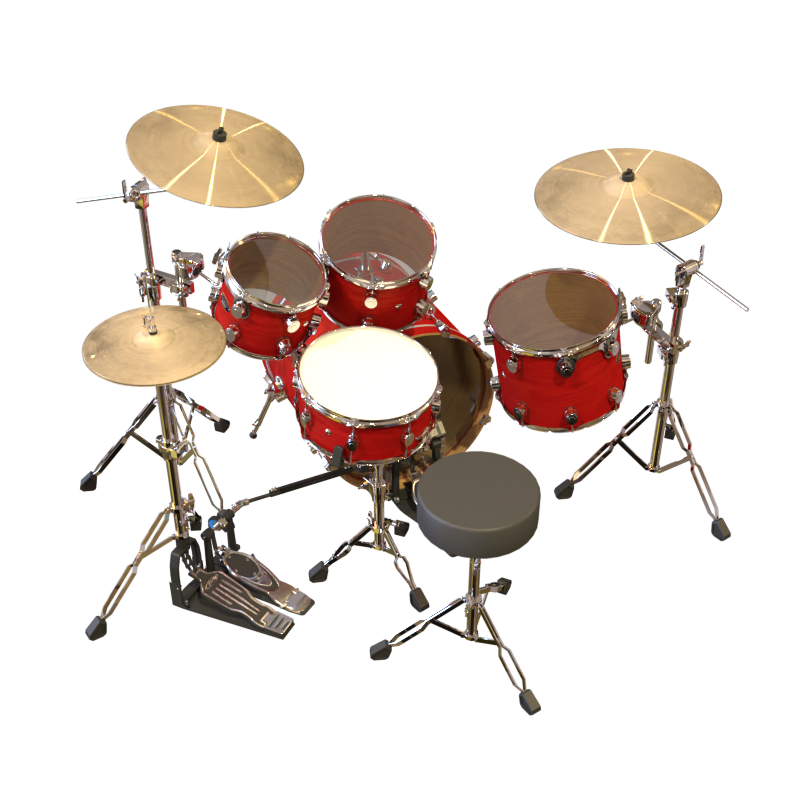
\includegraphics[width=.3\textwidth]{img/drums_gt.png}
				\medskip
				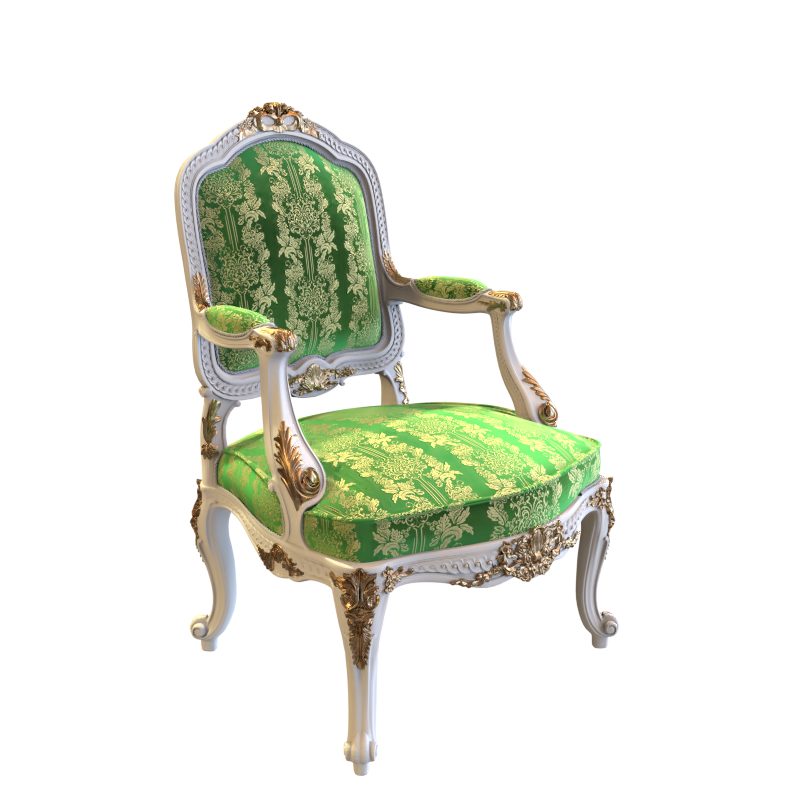
\includegraphics[width=.3\textwidth]{img/chair.png}\quad
				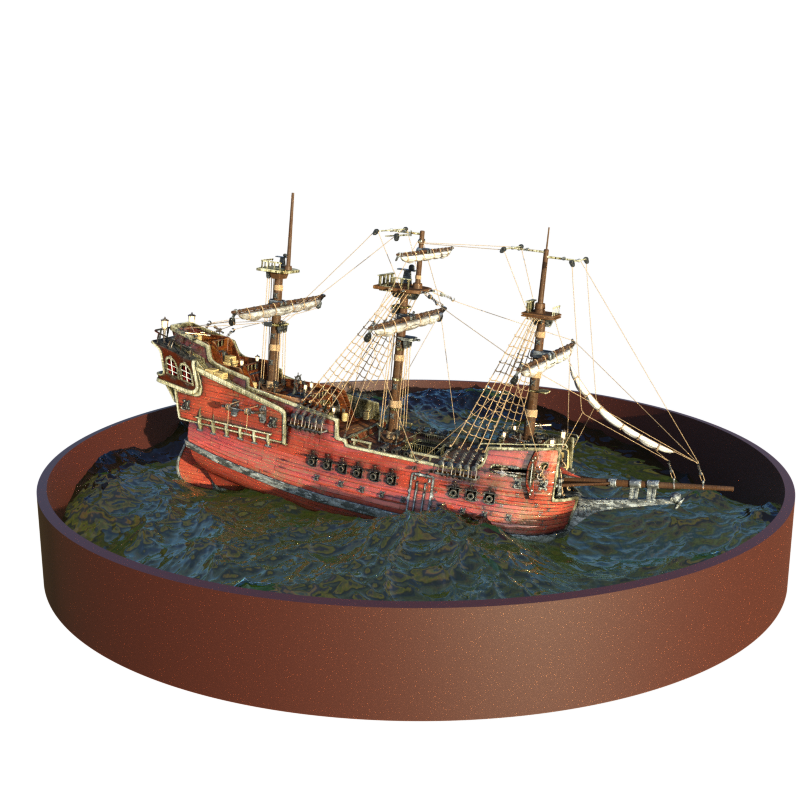
\includegraphics[width=.3\textwidth]{img/ship_gt.png}
				\caption{По један поглед из сваког скупа података}
				\label{fig-datasets}
			\end{figure}
		\end{frame}

	\section{Експерименти}
%		\begin{frame}{Метрике}
%			\begin{equation*}
%				\begin{split}
%					\text{PSNR} & = 10\log_{10}\left(\frac{I_{\max}^2}{\text{MSE}}\right) \\
%					\text{LPIPS} & = \sum_{l=1}^{L}\frac{1}{H_l W_l}\sum_{i=0}^{H_l - 1}\sum_{j=0}^{W_l - 1}
%					\left\Vert w_l \odot (\boldsymbol{\alpha}_{l; i, j}^{I} - \boldsymbol{\alpha}_{l; i, j}^{K}) \right\Vert^2 \\
%					\text{SSIM} & = \frac{(2\mu_{I}\mu_{K} + c_1)(2\sigma_{I, K} + c_2)}{(\mu_{I}^2 + \mu_{K}^2 + c_1)(\sigma_{I}^2 + \sigma_{K}^2 + c_2)}
%				\end{split}
%			\end{equation*}
%		\end{frame}
	
		\begin{frame}{Трошак обучавања}
			\begin{table}[H]
				\centering
				\begin{tabular}{cccc} \toprule
					{модел} 	& {време обучавања (у сатима)} & {број параметара} \\ \midrule
					{NeRF} 		& 120 						   & 1200000\\ 
					{mip-NeRF} 	& 127 						   & 612000\\
					{Ref-NeRF} 	& 135 						   & 1100000\\ \bottomrule
				\end{tabular}
			\end{table}
		\end{frame}
	
		\begin{frame}{Поређење}
			\begin{figure}
				\centering
				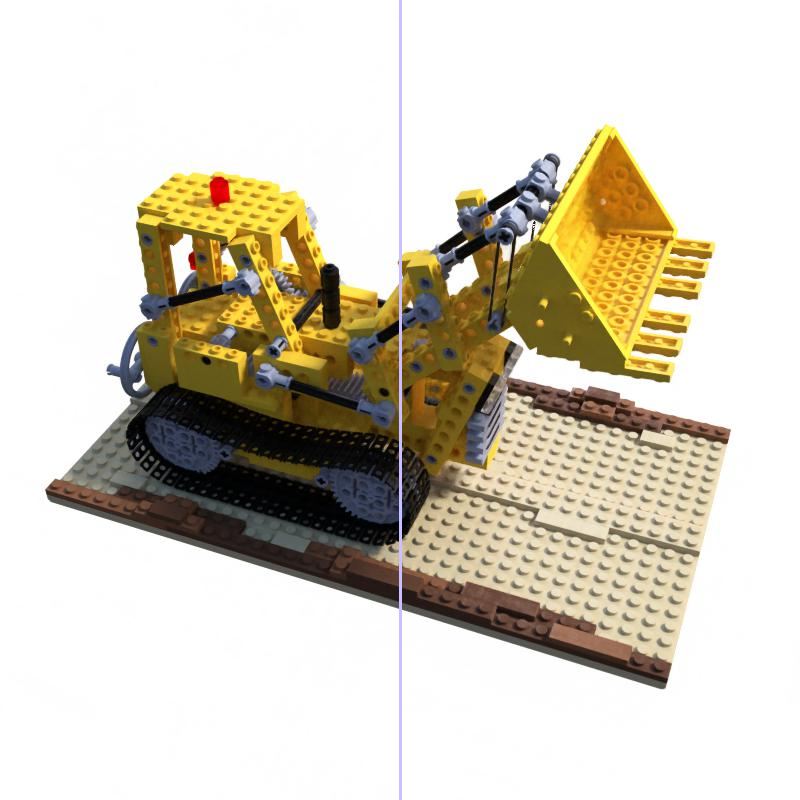
\includegraphics[width=0.5\textwidth]{img/comparison/mipnerf_vs_nerf_lego_31.png}
				\caption{NeRF | mip-NeRF}
			\end{figure}
		\end{frame}

		\begin{frame}{Поређење}
			\begin{figure}
				\centering
				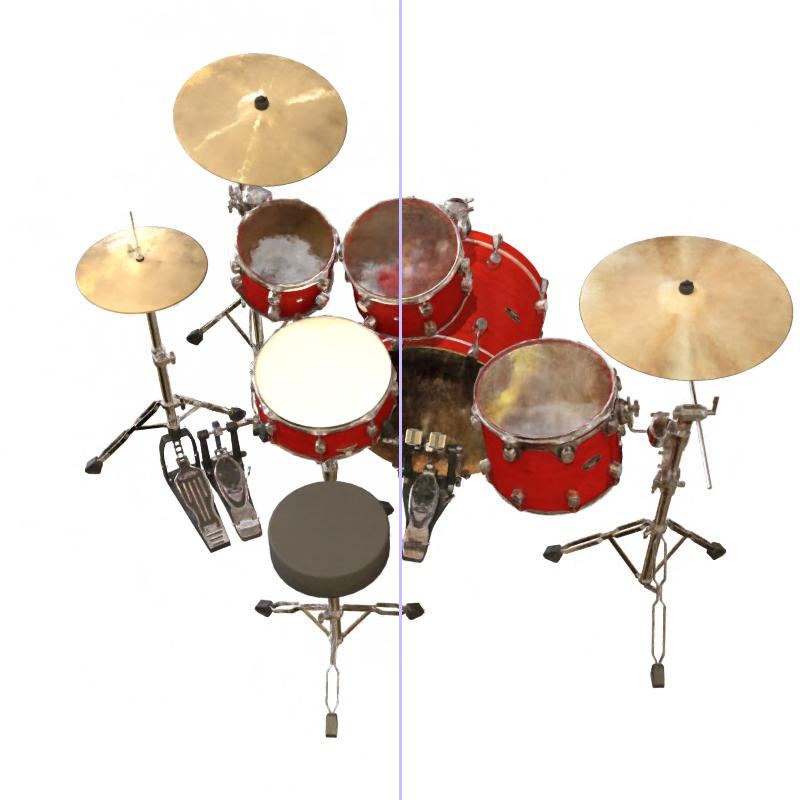
\includegraphics[width=0.5\textwidth]{img/comparison/refnerf_vs_mipnerf_drums_3.png}
				\caption{mip-NeRF | Ref-NeRF}
			\end{figure}
		\end{frame}

		\begin{frame}
			\begin{figure}
				\centering
				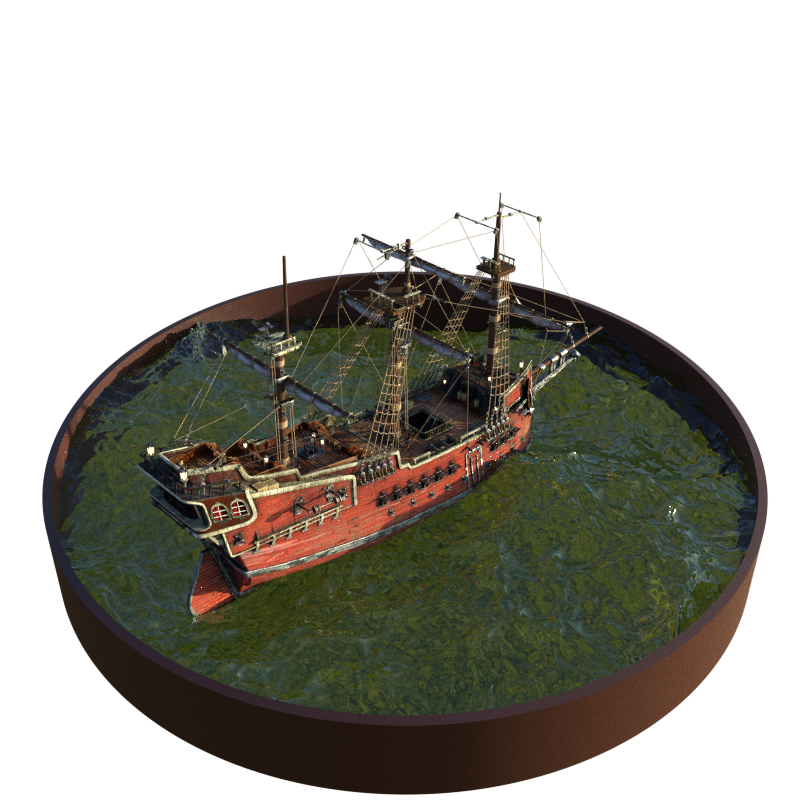
\includegraphics[width=0.45\textwidth]{img/comparison/gt_ship_38.png}\quad
				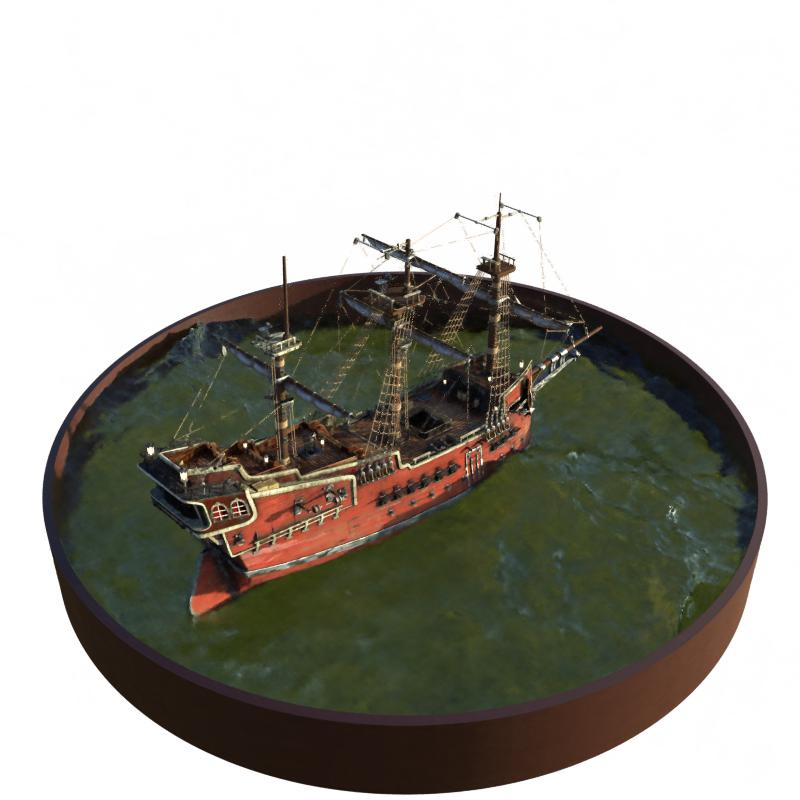
\includegraphics[width=0.45\textwidth]{img/comparison/refnerf_ship_38.jpg}
				\caption{GT и Ref-NeRF}
			\end{figure}
		\end{frame}

	\section{Закључак}
		\begin{frame}{Закључак}
			\begin{itemize}
				\item Квалитетни рендери
				\item Интерполација погледа
				\item Обучавање дуго траје
				\item Подржава само једну сцену
			\end{itemize}
		\end{frame}
	
		\begin{frame}{Даљи рад}
			\begin{itemize}
				\item Хијерархијски приступи
				\begin{itemize}
					\item InstantNGP (2022)
					\item ZipNeRF (2023)
				\end{itemize}
				\item Квантизација?
			\end{itemize}
		\end{frame}
\end{document}

